

% "draftfirst" or "draftall" as option to watermark, 10pt/11pt/12pt for font size, noextraspace if there are spacing issues, "man" for regular papers (assignments, journal submissions), jou for journal-esque formatting.
\documentclass[a4paper,man, 12pt]{apa6}

\usepackage[american]{babel}
\usepackage[utf8x]{inputenc}
\usepackage[amsmath]
\usepackage{csquotes}
\usepackage{graphicx}
\usepackage[style=apa,sortcites=true,sorting=nyt,backend=biber]{biblatex}

% Removes month from bibliography entries, which shouldn't be there for academic journals - optionally, remove the month entries from your .bib file on the offending files. Comment it out if using popular media, newspaper articles, etc. that need the month field. 
\AtEveryBibitem{
  \clearfield{month}
}
\DeclareLanguageMapping{american}{american-apa}

% Removes "retrieved from on date" from bibliography entry unless it is a wiki URL, which is closer to the spirit of APA's rule. See biblatex-apa documentation for more info.
\DeclareSourcemap{
\maps[datatype=bibtex]{
\map{
\step[fieldsource=url,
notmatch=\regexp{wiki},
final=1]
\step[fieldset=urldate, null]
}
}
}

% Add your BibTeX files here. Use source location if you aren't keeping them as the same folder as your document.
\addbibresource{bibsource}
%    \bibliography{main}
%    \bibliographystyle{plain}


% Can help catch outdated code practices by giving you console warnings. Commented out by default so as to not confuse new users.
%\usepackage[l2tabu]{nag}

% title, etc.
\title{ITCO620 Individual Project Unit 1}
\shorttitle{ITCO620 INDIVIDUAL PROJECT UNIT 1}
\author{NaDario M. Seays Sr}

% The following four fields make up some of the front matter of your document. If working on an assignment for a course, I typically use "affiliation" for the class name. I have commented out abstract since minimal usage doesn't require it and leaving it blank will generate a blank page. Ignore the warning about the lack of abstract. 

\affiliation{American Inter-Continental University}
\abstract{Your abstract here.}
%\keywords{}
%\authornote{}

\begin{document}
\maketitle

\section{Introduction}

Your introduction goes here! Some examples of commonly used commands and features are listed below, to help you get started.

If you have a question, please use the support box in the bottom right of the screen to get in touch.

\section{Some \LaTeX{} Examples}
\label{sec:examples}

\subsection{Sections}

Use section and subsection commands to organize your document. \LaTeX{} handles all the formatting and numbering automatically. Use ref and label commands for cross-references.

\subsection{Comments}

You can add inline TODO comments with the todonotes package, like this:
\todo[inline, color=green!40]{This is an inline comment.}

\subsection{References}

LaTeX automatically generates a bibliography in the APA style from your .bib file. The citep command generates a formatted citation in parentheses \citep{Lamport1986}. The cite command generates one without parentheses. LaTeX was first discovered by \cite{Lamport1986}.

\subsection{Tables and Figures}

Use the table and tabular commands for basic tables --- see Table~\ref{tab:widgets}, for example. You can upload a figure (JPEG, PNG or PDF) using the files menu. To include it in your document, use the includegraphics command as in the code for Figure~\ref{fig:frog} below.

% Commands to include a figure:
\begin{figure}
\centering
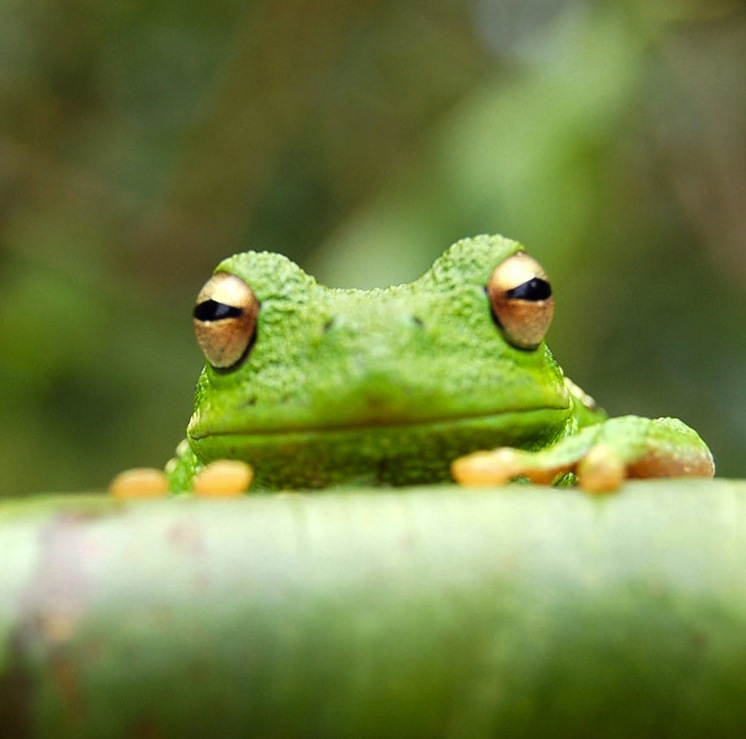
\includegraphics[width=0.5\textwidth]{frog.jpg}
\caption{\label{fig:frog}This is a figure caption.}
\end{figure}

\begin{table}
\centering
\begin{tabular}{l|r}
Item & Quantity \\\hline
Widgets & 42 \\
Gadgets & 13
\end{tabular}
\caption{\label{tab:widgets}An example table.}
\end{table}

\subsection{Mathematics}

\LaTeX{} is great at typesetting mathematics. Let $X_1, X_2, \ldots, X_n$ be a sequence of independent and identically distributed random variables with $\text{E}[X_i] = \mu$ and $\text{Var}[X_i] = \sigma^2 < \infty$, and let
$$S_n = \frac{X_1 + X_2 + \cdots + X_n}{n}
      = \frac{1}{n}\sum_{i}^{n} X_i$$
denote their mean. Then as $n$ approaches infinity, the random variables $\sqrt{n}(S_n - \mu)$ converge in distribution to a normal $\mathcal{N}(0, \sigma^2)$.

\subsection{Lists}

You can make lists with automatic numbering \dots

\begin{enumerate}
\item Like this,
\item and like this.
\end{enumerate}
\dots or bullet points \dots
\begin{itemize}
\item Like this,
\item and like this.
\end{itemize}

We hope you find write\LaTeX\ useful, and please let us know if you have any feedback using the help menu above.

\bibliography{example}

% This is where the bibliography goes. Finish the body of your paper before this point, other than the appendix. 
%\printbibliography

% I have commented out the appendix section since it isn't a standard for minimal documents. 
%\appendix 

\end{document}
